\chapter{Resultats}


\label{Chap-Res}

\section{État fondamental du calcium oxalate}
\subsection{Structure moléculaire}
%TODO add reference
La cellule élémentaire de calcium oxalate ($Ca C_2 O_4$) contient 28 atomes. Il est de structure monoclique et de groupe de symétrie $P2/m$ ($\#$10) (cf. figure \ref{BrillouinZone})
%TODO add bilbao

\begin{figure}[!h]\label{BrillouinZone}
    \centering
    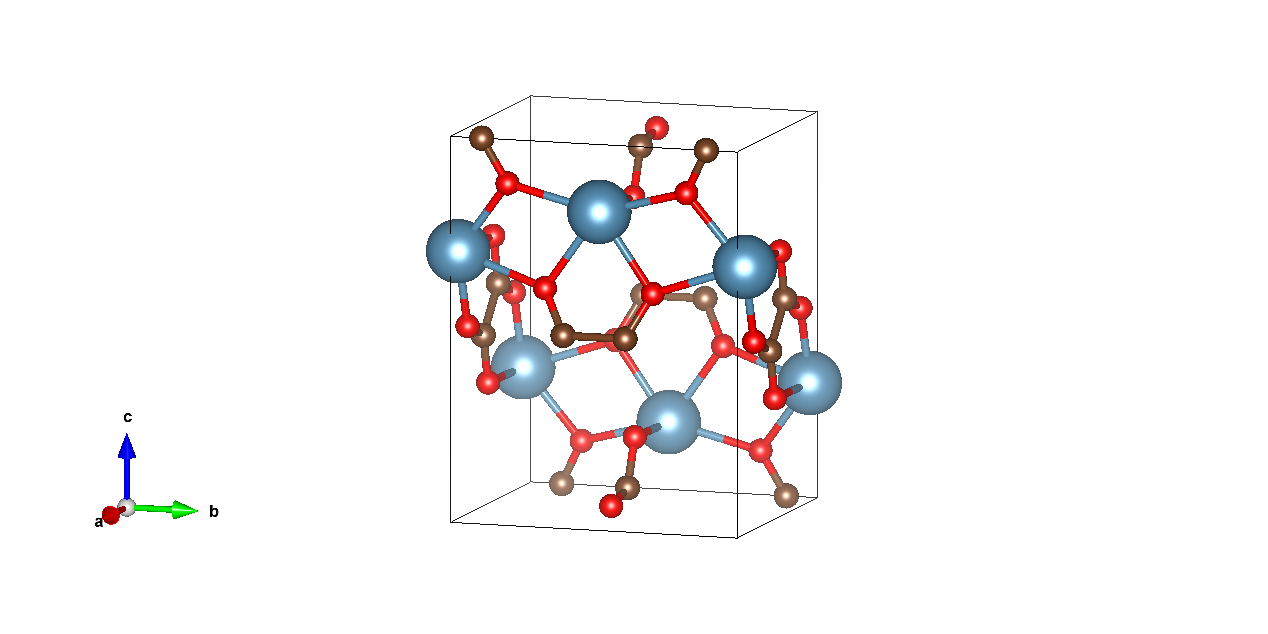
\includegraphics[width=20cm]{co_structure}
    \caption{La cellule élémentaire de l'oxalate de calcium}
\end{figure}
%%%%%%%%%%%%%%%%%%%%%%%%%%%%%%%%%%%%%%%%%
\subsection{Énergie de seuil}
Pour commencer, on étudie la convergence du calcul de l'état fondamental de calcium oxalate. On fait varier le seuil d'énergie $E_{cut}$ entre 20 et 100 Hatree. 
On constate que pour tous ces seuils d'énergies, on obtient bien une convergence au bout de 15 itérations. La relation entre l'énergie totale du système à la convergence en fonction de l'énergie de seuil est tracée dans la figure \ref{Ecut}. 
À partir de $E_{cut} = 40$ Hatree, l'énergie totale du système est bien minimisée. On choisit donc cette énergie de seuil pour la suite du calcul de l'état fondamental. 

\begin{figure}[!h]\label{Ecut}
    \centering
    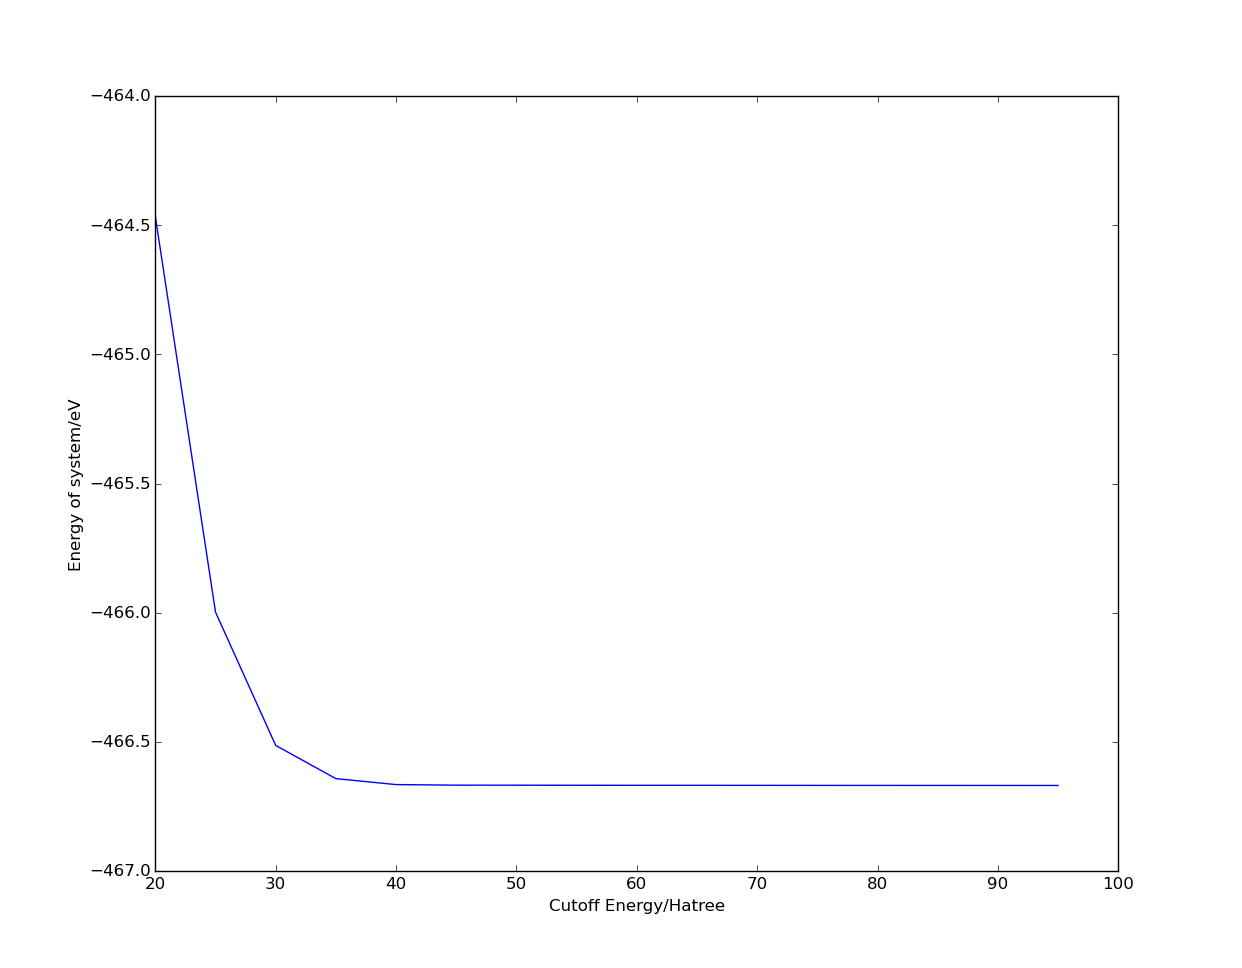
\includegraphics[width=12cm]{E_cut}
    \caption{Ecut}
\end{figure}

%Dans un premier temps, avant de passer à l'état exicité, on peut construire sa structure de bandes à l'aide du calcul d'Abinit (cf. figure \ref{BrillouinZone}). 
%Il est à remarquer que la structure de bande des états exicités seront différents que celle de l'état fondamental. 
%Cependant, on pourrait avoir des idées sur celle des états excités. 
%Notamment, le gap de la structure de bande montre que le calcium oxalate n'est pas un conducteur. 
%Par ailleurs, comme le gap n'est pas direct, on peut donc observer des lumières émises dans des directions non parallèles à la lumière incidente. 
%%%%%%%%%%%%%%%%%%%%%%%%%%%%%%%%%%%%%%%%%%%%%%%
\section{Spectres de perte d'énergie (EELS)}
%%%%%%%%%%%%%%%%%%%%%%%%%%%%%%%%%%%%%%%%%%%%%%%%
\subsection{Convergence avec les points-k}
La motivation de ce test de convergence est de pouvoir avoir un échantillonnage assez fin pour obtenir tous les états d'excitation possibles sans avoir trop de points-k, ce qui augmentera considérablement la compléxité du calcul.
Même si les calculs de convergence avec les nombres de points-k différents ont été faits pour l'état fondamental, il faut s'assurer que l'échantillonnage que l'on a privilégié soit aussi assez fin pour les calculs de réponse de la matériau sous une excitation extérieure. 
On crée des fichiers décrivant la densité de l'état fondamental avec des échantillonnages de la première zone de Brillouin différents, où dans la première zone de Brouillin, il y a respectivement 16, 120 et 480 points-k. 
Pour connaître le meilleur échantillonnage à utiliser à notre disposition, on fait d'abord les calculs en prenant RPA (ramdom phase approximation) comme méthode d'approximation du terme d'échange et de corrélation.
On montre dans la figure \ref{kptCompare} que le choix du 120 points-k dans la première zone de Brillouin donne déjà de bons résultats pour le calcul de EELS (par rapport à 480 points-k). On peut donc se contenter de prendre l'échantillonnage avec 120 points-k pour la suite du calcul.

%%%%%%%%%%%%%%%%%%%%%%%%%%%%%%%%%%%%%%%%%%%%%%%%%%%%%%%
\subsection{Convergence avec les bandes}

\begin{figure}[!h]\label{cv_nbd}
    \centering
    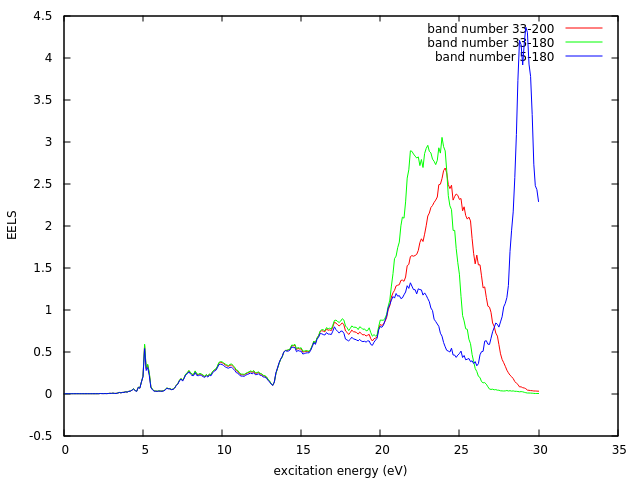
\includegraphics[width=12cm]{nbd_compare}
    \caption{Convergence en bande}
\end{figure}

Pour le calcul de $\epsilon^{-1}$ (l'inverse de la fonction diélectrique, qui servira à calculer EELS), il faut passer par le calcul de la fonction de réponse linéaire (cf. Annexe \ref{TRL}). 
Pour ce calcul, on doit considérer toutes les transitions possibles (excitation d'un électron de la bande de valence vers une bande de conduction). 
Il est donc nécessaire de converger le calcul de EELS par rapport au nombre de bandes de valence et de conduction (cf. \ref{chi}). 
Le but est de considérer seulement les transitions pour les énergies qui nous intéressent afin de gagner en temps de calcul sans perdre des informations. 
Nous nous intéressons notamment aux transitions en basse énergie (< 20 eV).
Le résultat montré dans la figure \ref{cv_nbd} montre qu'il suffit de prendre en compte les transitions entre la bande remplie numéro 33 (en comptant à partir de la bande d'énergie la plus basse) et la bande numéro 180. 

%%%%%%%%%%%%%%%%%%%%%%%%%%%%%%%%%%%%%%%%%%%%%%

\subsection{RPA vs ALDA}
La méthode d'approximation du terme d'échange et de corrélation RPA prend moins de temps pour le calcul mais pourrait perdre la précision. Il est donc judicieux de comparer les résultats obtenus en appliquant RPA avec ceux obtenus en appliquant ALDA (adiabatic local density approximation).
Les deux approximations nous donnent des résultats assez proches en basses énergies.
Dans le cadre de ce projet, on se contente d'étudier les caractéristiques de calcium oxalate en basse énergie en raison du délai.
Il est donc tout à fait pertinent de faire notre calcul en RPA pour gagner en temps de calcul.
\begin{figure}[!h]
    \centering
    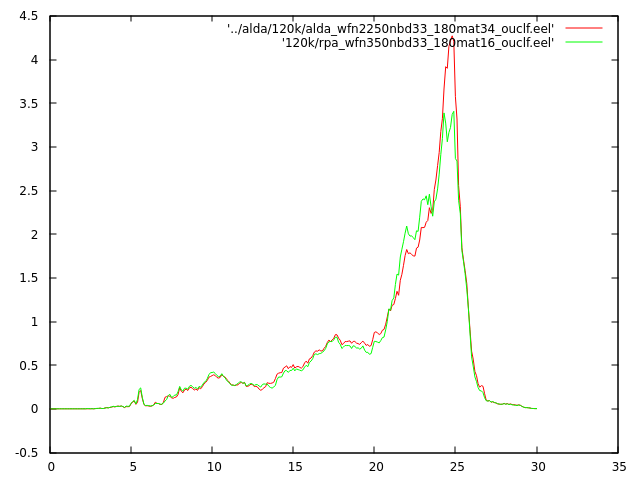
\includegraphics[width=8cm]{alda_vs_rpa}
    \caption{alda}
\end{figure}
%%%%%%%%%%%%%%%%%%%%%%%%%%%%%%%%%%%%%%%%%%%%%%%
\subsection{Anisotropie du système}

\begin{figure}[!h]\label{anisotropie}
    \centering
    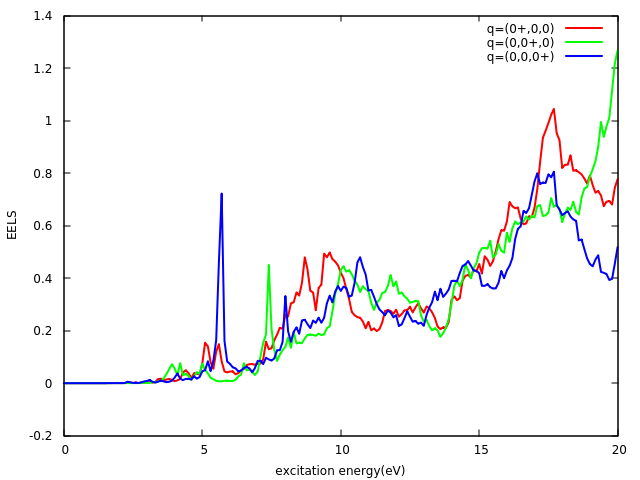
\includegraphics[width=12cm]{anisotropy}
    \caption{L'anisotropie du système}
\end{figure}

Cette étude consiste à examiner l'isotropie du système. 
En effet, les transitions peuvent avoir lieu dans les directions différentes. 
Un électron peut changer son vecteur d'onde en allant d'une bande à une autre. 
Ce type de transition est pris en compte dans la formule \ref{chi_q} qui nous donne la polarizabilité que l'on est censé observer dans une direction donnée (\textbf{q} dans l'expression \ref{chi_q})
Or, comme certains termes sont négligés dans le calcul numérique, on peut avoir des valeurs différentes en $q = 0$ en fonction de la direction par laquelle on s'y rapproche.
Les calculs de EELS en $q = 0$ selon les trois axes (par exemple, $q=(0+,0,0)$ pour le premier axe de la zone de Brillouin) sont montrés dans la figure \ref{anisotropie}
La différence entre les différentes valeurs trouvées est dûe à l'anisotropie de la structure.  
%%%%%%%%%%%%%%%%%%%%%%%%%%%%%%%%%%%%%%%%%%%%%%%%
%picture missing
\subsection{EELS et la fonction diélectrique}
\begin{figure}[!h]\label{dispersion}
    \centering
    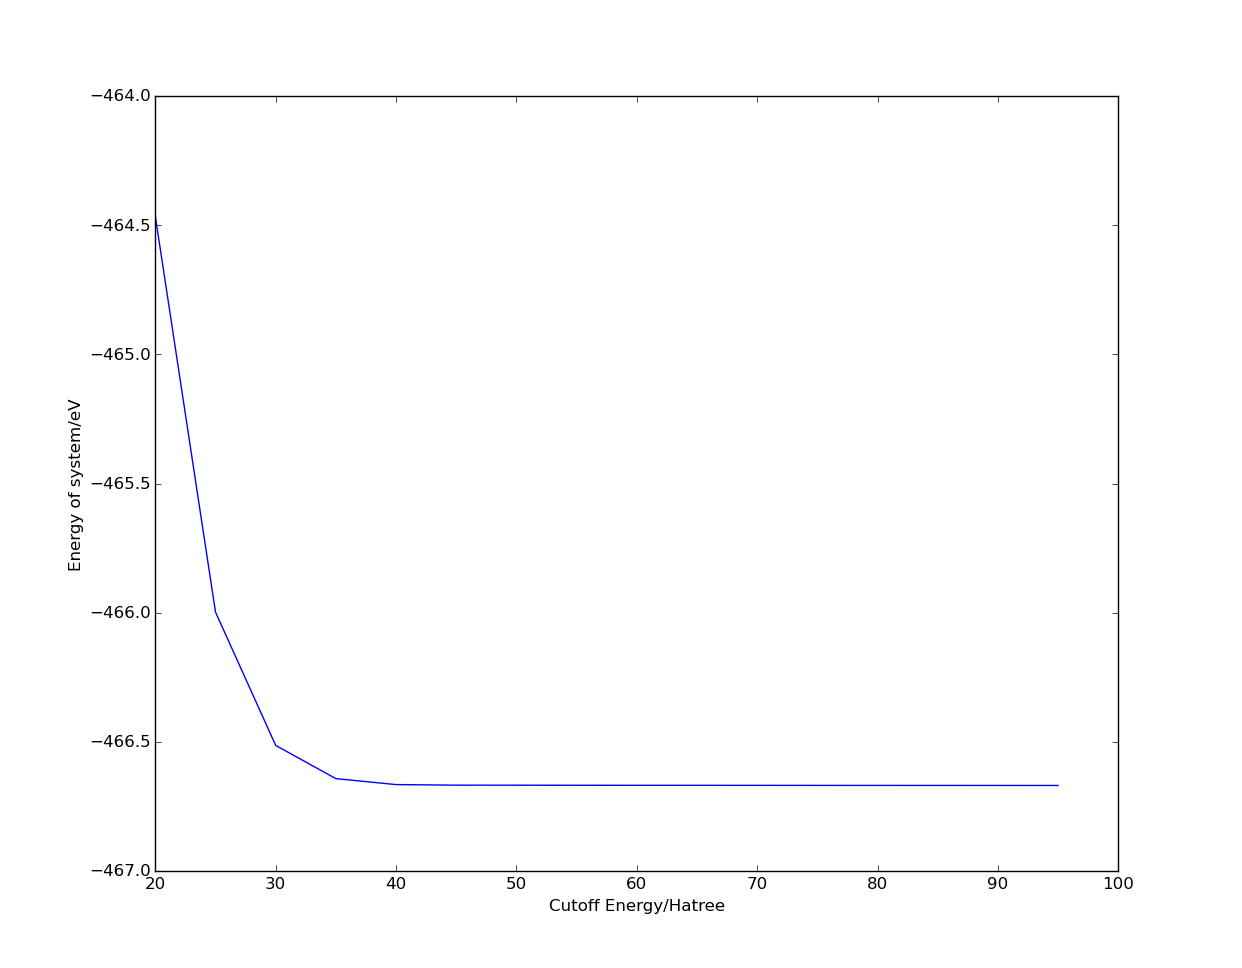
\includegraphics[width=12cm]{E_cut}
    \caption{Ecut}
\end{figure}

%%%%%%%%%%%%%%%%%%%%%%%%%%%%%%%%%%%%%%%%%%%%%%%%%%%
\subsection{Dispersion}
Enfin, on s'intéresse à la dispersion des spectres EELS. 
Il s'agit de changer la valeur de \textbf{q} dans la formule \ref{chi_q} (non proche de 0 cette fois-ci).
Il est intéressant de remarquer que la stabilité de la position du premier pique de résonance pour les trois différentes directions de dispersion (fig. \ref{q6}, \ref{q8} et \ref{q10}).
Bien que la valeur de EELS obtenue pour le premier pique change en fonction de \textbf{q}, le pique se trouve toujours en même énergie d'excitation quand on fait varier la valeur de \textbf{q} dans une direction donnée. 
\\\\
Dans une vraie expérience, on est limité par la résolution des l'appareils.
Il est donc difficile à déterminer, en général, si une réponse forte est due à une résonance ou à une superposition de réponses pour différentes valeurs de \textbf{q}.
Pour l'oxalate de calcium, un expérimentateur pourra se convaincre que la réponse qu'il obtiendra pour une énergie qui correspond à un pique de EELS est une vraie résonance.


\begin{figure}[!h]\label{q6}
    \centering
    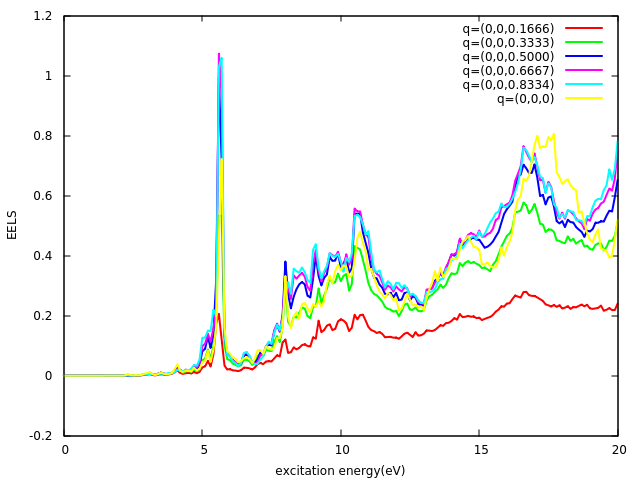
\includegraphics[width=12cm]{q6}
    \caption{EELS pour différents \textbf{q} dans la direction (0, 0, 1) de la première de Brillouin}
\end{figure}

\begin{figure}[!h]\label{q8}
    \centering
    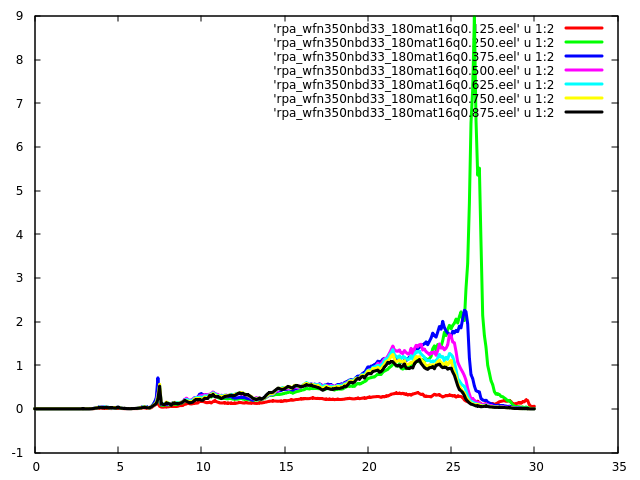
\includegraphics[width=12cm]{q8}
    \caption{EELS pour différents \textbf{q} dans la direction (0, 1, 0) de la première de Brillouin}
\end{figure}
\begin{figure}[!h]\label{q10}
    \centering
    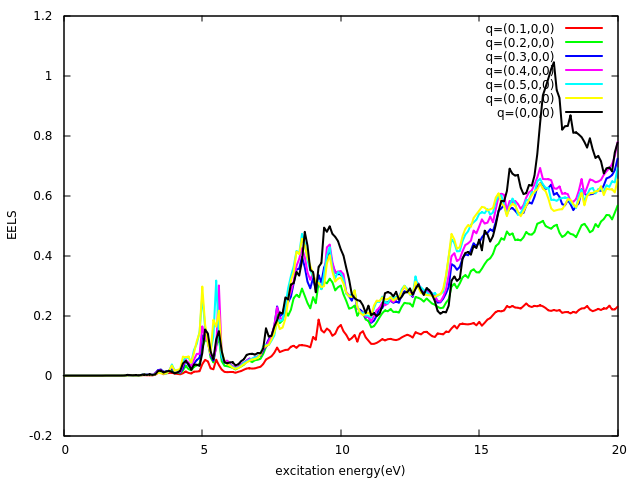
\includegraphics[width=12cm]{q10}
    \caption{EELS pour différents \textbf{q} dans la direction (1, 0, 0) de la première de Brillouin}
\end{figure}